\section{Forward Kinematics}
\emph{Forward kinematics} allows to compute the position and orientation of the kinematic chain given the joint parameters (e.g. angles, lengths, etc.). For instance, we can compute the position and orientation of the terminal organ given the angles of the articulations.
\begin{figure}[H]
    \centering
    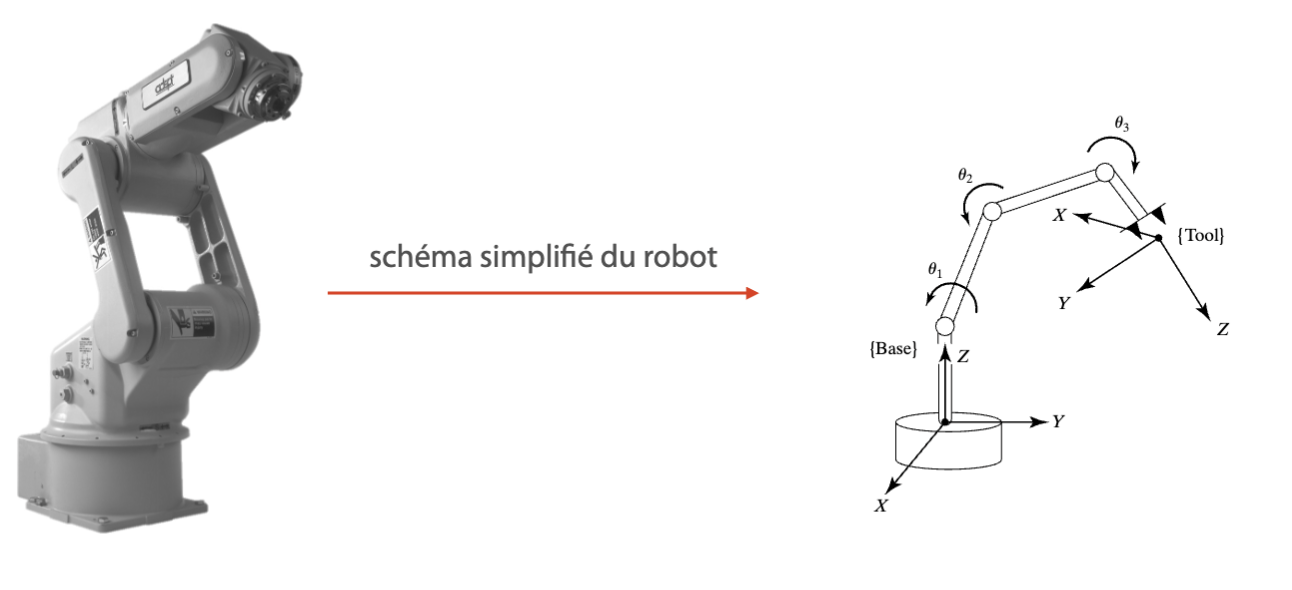
\includegraphics[width=.7\textwidth]{position/direct-kinematic.png}
\end{figure}

The kinematic chain is composed of rigid bodies interconnect by joints. The joins define the degrees of freedom of the cinematic chain, which are the parameters that we can control.
\begin{figure}[H]
    \centering
    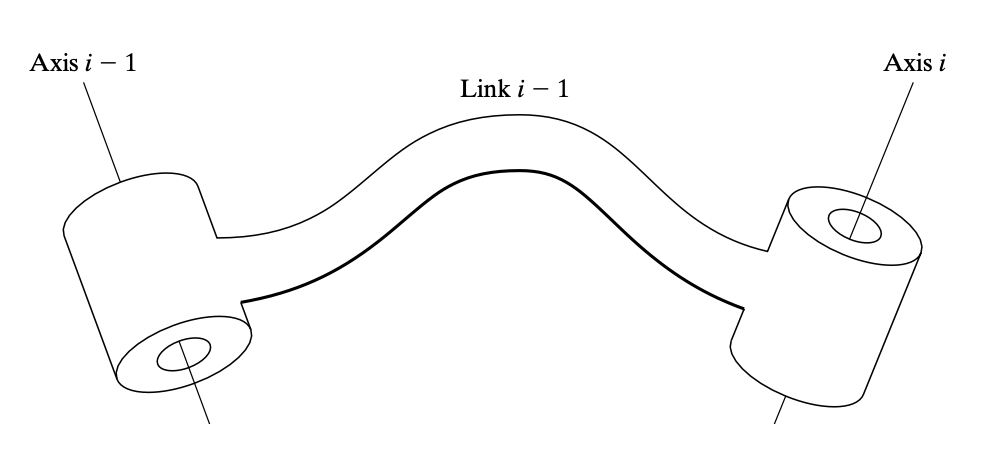
\includegraphics[width=.5\textwidth]{forward-kinematics/kinematic-chain.png}
\end{figure}

\subsection{Articulations and joint speed}
\subsubsection{Joint types and degrees of freedom}
The topology of the articulation between two rigid bodies defines the degrees of freedom of the joint.
\begin{figure}[H]
    \centering
    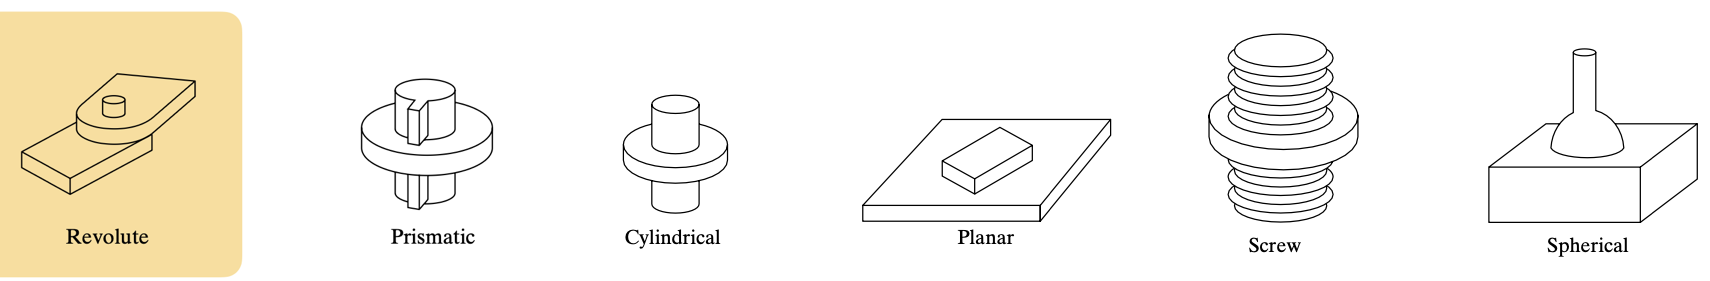
\includegraphics[width=.9\textwidth]{forward-kinematics/joints.png}
    \caption{Example of possible joints.}
\end{figure}
Each joint can be represented as a function $K_i$ from a configuration space $Q_i$ to the Special Euclidean Group $\SE(3)$:
\begin{equation*}
    \begin{aligned}
        K_i: Q_i &\longrightarrow \SE(3)\\
        q &\longmapsto M_i(q_i)
    \end{aligned}
\end{equation*}

Consider for instance the revolute joint, which constrains the motion of two bodies around a fixed axis. It is parameterized by the angle $\theta\in\R$, therefore the configuration space is $Q_i=\Sb^1\simeq\R$ (one degree of freedom). The function $K_i$ is then defined as:
\begin{equation*}
    \begin{aligned}
        K_i: \Sb^1\simeq\R &\longrightarrow \SE(3)\\
        q &\longmapsto \begin{bmatrix}
            \cos  & -\sin q & 0 & 0\\
            \sin q & \phantom{-}\cos q & 0 & 0\\
            0 & 0 & 1 & 0\\
            0 & 0 & 0 & 1
        \end{bmatrix}
    \end{aligned}
\end{equation*}

\subsubsection{Joint speed}
The change of configuration of the joint comes from the joint speed, which is the derivative of the joint parameter with respect to time. Consider the relative position of the articulation between the two adjacent frames, given by:
\begin{equation*}
    \begin{aligned}
        K_i : Q_i &\longrightarrow \SE(3)\\
        q_i &\longmapsto M_i(q_i)
    \end{aligned}
\end{equation*}
The relative speed of the joint generated by the articulation is given by:
\begin{equation*}
    \begin{aligned}
        k_i:T_{q_i}Q_i &\longrightarrow \se(3)\\
        (q_i, \dot{q}_i) &\longmapsto v_i(q_i) = S_i(q_i)\dot{q}_i
    \end{aligned}
\end{equation*}
for some transformation $S_i$.

In the case of the revolute joint, the speed of the joint is given by:
\begin{equation*}
    \begin{aligned}
        k_i: T_q\Sb^1\simeq\R^2 &\longrightarrow \se(3)\\
        (q, \dot{q}) &\longmapsto (v, w) = \left(
            \begin{bmatrix}
                0\\0\\0
            \end{bmatrix}, \begin{bmatrix}
                0\\0\\\dot{q}
            \end{bmatrix}\right)
    \end{aligned}
\end{equation*}
Hence, we have:
\begin{equation*}
    S_i(q) = \begin{bmatrix}
        0\\0\\0\\0\\0\\1
    \end{bmatrix} \in \mathscr{M}_{6, 1}(\R)
\end{equation*}
which gives us $S_i(q)\dot{q}=(v,w)$ as expected.

\subsection{Direct geometry}
We aim to compute the position and orientation of the terminal organ given the joint parameters. We can do so by computing the transformation matrix of each body in the kinematic chain, and then multiplying them to get the transformation matrix of the terminal organ.

\subsubsection{Transformation matrix}
Given an articulation $i$, we can compute the relative position of the associated frame $i$ with respect to the frame $i-1$ using the function $K_i$:
\begin{equation*}
    \prescript{i-1}{}{M_i(q_i)} = \prescript{i-1}{}{P_iK_i(q_i)}
\end{equation*}
We can combine the transformations of all the bodies in the kinematic chain to get the transformation matrix of the terminal organ:
\begin{equation*}
    \begin{aligned}
        \prescript{0}{}{K_n} : \bigtimes_{i=1}^n Q_i &\longrightarrow \SE(3)\\
        q=(q_1, \dots, q_n) &\longmapsto \bigtimes_{i=1}^n \prescript{i-1}{}{M_i(q_i)}
    \end{aligned}
\end{equation*}
Therefore, the configuration space can be read as the product of the configuration spaces of each joint:
\begin{equation*}
    Q = \bigtimes_{i=1}^N Q_i \simeq \R^{\sum_{i=1}^N n_i}
\end{equation*}
where $N$ is the number of joints.

\subsubsection{Kinematic Jacobian}
Our goal is now to link the joint speed to the spatial speed of the bodies in movement. For each articulation, we have a linear mapping of the form:
\begin{equation*}
    v_i(q_i) = S_i(q_i)\dot{q_i}
\end{equation*}
This corresponds to the temporal derivative of the articular geometry:
\begin{equation*}
    \dot{M}_i(q_i)M_i^{-1}(q_i) = S_i(q_i)\dot{q}_i
\end{equation*}
Therefore, one can link the spatial speed of a body to the joint speed using the relation:
\begin{equation*}
    \prescript{0}{}{k_n}(q, \dot{q}) = \sum_{i=1}^n k_i(q_i, \dot{q}_i) = \underbrace{\begin{bmatrix}
        S_1(q_1) \cdots S_n(q_n)
    \end{bmatrix}}_{J(q)}
    \begin{bmatrix}
        \dot{q}_1\\\vdots\\\dot{q}_n
    \end{bmatrix}
\end{equation*}